% Created by tikzDevice version 0.6.1 on 2011-06-03 22:21:25
% !TEX encoding = UTF-8 Unicode
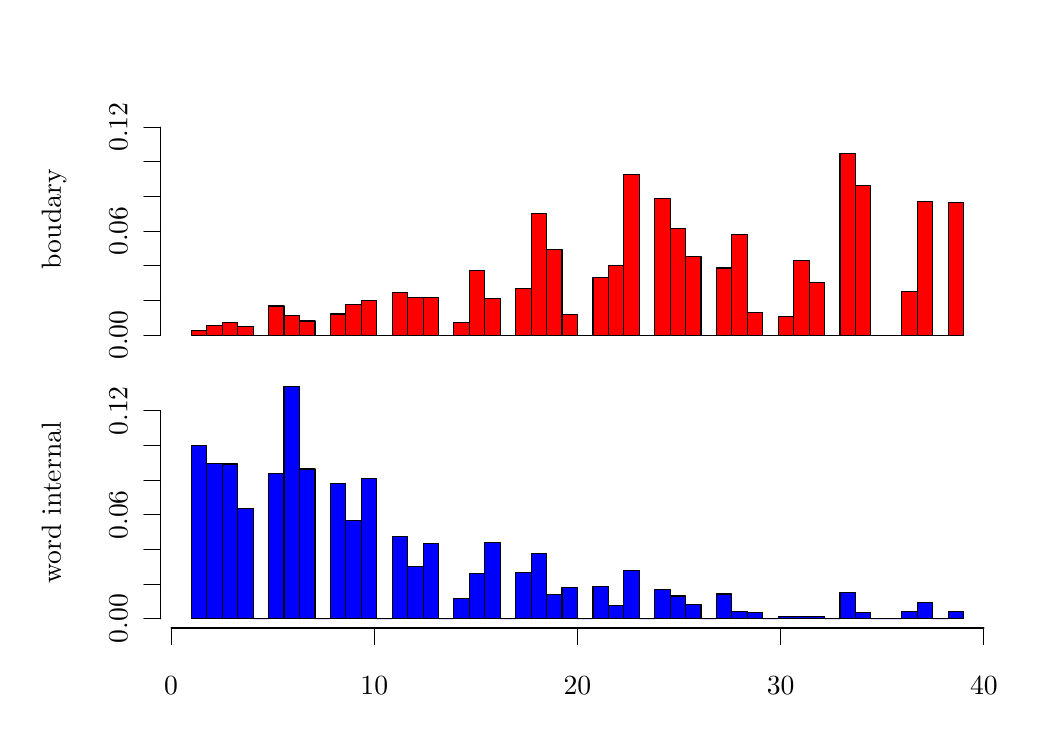
\begin{tikzpicture}[x=1pt,y=1pt]
\definecolor[named]{drawColor}{rgb}{0.00,0.00,0.00}
\definecolor[named]{fillColor}{rgb}{1.00,1.00,1.00}
\fill[color=fillColor,] (0,0) rectangle (361.35,252.94);
\begin{scope}
\path[clip] (  0.00,126.47) rectangle (361.35,252.94);
\definecolor[named]{drawColor}{rgb}{0.78,0.56,0.83}
\definecolor[named]{drawColor}{rgb}{0.00,0.00,0.00}

\node[rotate= 90.00,color=drawColor,anchor=base,inner sep=0pt, outer sep=0pt, scale=  1.00] at ( 12.00,183.71) {boudary%
};
\end{scope}
\begin{scope}
\path[clip] (  0.00,  0.00) rectangle (361.35,252.94);
\definecolor[named]{drawColor}{rgb}{0.78,0.56,0.83}
\definecolor[named]{drawColor}{rgb}{0.00,0.00,0.00}

\draw[color=drawColor,line cap=round,line join=round,fill opacity=0.00,] ( 48.00,141.82) -- ( 48.00,216.97);

\draw[color=drawColor,line cap=round,line join=round,fill opacity=0.00,] ( 48.00,141.82) -- ( 42.00,141.82);

\draw[color=drawColor,line cap=round,line join=round,fill opacity=0.00,] ( 48.00,154.35) -- ( 42.00,154.35);

\draw[color=drawColor,line cap=round,line join=round,fill opacity=0.00,] ( 48.00,166.87) -- ( 42.00,166.87);

\draw[color=drawColor,line cap=round,line join=round,fill opacity=0.00,] ( 48.00,179.40) -- ( 42.00,179.40);

\draw[color=drawColor,line cap=round,line join=round,fill opacity=0.00,] ( 48.00,191.92) -- ( 42.00,191.92);

\draw[color=drawColor,line cap=round,line join=round,fill opacity=0.00,] ( 48.00,204.45) -- ( 42.00,204.45);

\draw[color=drawColor,line cap=round,line join=round,fill opacity=0.00,] ( 48.00,216.97) -- ( 42.00,216.97);

\node[rotate= 90.00,color=drawColor,anchor=base,inner sep=0pt, outer sep=0pt, scale=  1.00] at ( 36.00,141.82) {0.00%
};

\node[rotate= 90.00,color=drawColor,anchor=base,inner sep=0pt, outer sep=0pt, scale=  1.00] at ( 36.00,179.40) {0.06%
};

\node[rotate= 90.00,color=drawColor,anchor=base,inner sep=0pt, outer sep=0pt, scale=  1.00] at ( 36.00,216.97) {0.12%
};
\end{scope}
\begin{scope}
\path[clip] ( 48.00,138.47) rectangle (349.35,228.94);
\definecolor[named]{drawColor}{rgb}{0.78,0.56,0.83}
\definecolor[named]{drawColor}{rgb}{0.00,0.00,0.00}
\definecolor[named]{fillColor}{rgb}{1.00,0.00,0.00}

\draw[color=drawColor,line cap=round,line join=round,fill=fillColor,] ( 59.16,141.82) rectangle ( 64.74,143.40);

\draw[color=drawColor,line cap=round,line join=round,fill=fillColor,] ( 64.74,141.82) rectangle ( 70.32,145.20);

\draw[color=drawColor,line cap=round,line join=round,fill=fillColor,] ( 70.32,141.82) rectangle ( 75.90,146.39);

\draw[color=drawColor,line cap=round,line join=round,fill=fillColor,] ( 75.90,141.82) rectangle ( 81.48,145.08);

\draw[color=drawColor,line cap=round,line join=round,fill=fillColor,] ( 81.48,141.82) rectangle ( 87.06,141.82);

\draw[color=drawColor,line cap=round,line join=round,fill=fillColor,] ( 87.06,141.82) rectangle ( 92.64,152.38);

\draw[color=drawColor,line cap=round,line join=round,fill=fillColor,] ( 92.64,141.82) rectangle ( 98.22,148.85);

\draw[color=drawColor,line cap=round,line join=round,fill=fillColor,] ( 98.22,141.82) rectangle (103.81,146.93);

\draw[color=drawColor,line cap=round,line join=round,fill=fillColor,] (103.81,141.82) rectangle (109.39,141.82);

\draw[color=drawColor,line cap=round,line join=round,fill=fillColor,] (109.39,141.82) rectangle (114.97,149.47);

\draw[color=drawColor,line cap=round,line join=round,fill=fillColor,] (114.97,141.82) rectangle (120.55,153.00);

\draw[color=drawColor,line cap=round,line join=round,fill=fillColor,] (120.55,141.82) rectangle (126.13,154.50);

\draw[color=drawColor,line cap=round,line join=round,fill=fillColor,] (126.13,141.82) rectangle (131.71,141.82);

\draw[color=drawColor,line cap=round,line join=round,fill=fillColor,] (131.71,141.82) rectangle (137.29,157.27);

\draw[color=drawColor,line cap=round,line join=round,fill=fillColor,] (137.29,141.82) rectangle (142.87,155.49);

\draw[color=drawColor,line cap=round,line join=round,fill=fillColor,] (142.87,141.82) rectangle (148.45,155.54);

\draw[color=drawColor,line cap=round,line join=round,fill=fillColor,] (148.45,141.82) rectangle (154.03,141.82);

\draw[color=drawColor,line cap=round,line join=round,fill=fillColor,] (154.03,141.82) rectangle (159.61,146.29);

\draw[color=drawColor,line cap=round,line join=round,fill=fillColor,] (159.61,141.82) rectangle (165.19,165.31);

\draw[color=drawColor,line cap=round,line join=round,fill=fillColor,] (165.19,141.82) rectangle (170.77,155.19);

\draw[color=drawColor,line cap=round,line join=round,fill=fillColor,] (170.77,141.82) rectangle (176.35,141.82);

\draw[color=drawColor,line cap=round,line join=round,fill=fillColor,] (176.35,141.82) rectangle (181.93,158.82);

\draw[color=drawColor,line cap=round,line join=round,fill=fillColor,] (181.93,141.82) rectangle (187.51,185.76);

\draw[color=drawColor,line cap=round,line join=round,fill=fillColor,] (187.51,141.82) rectangle (193.09,172.69);

\draw[color=drawColor,line cap=round,line join=round,fill=fillColor,] (193.09,141.82) rectangle (198.67,149.25);

\draw[color=drawColor,line cap=round,line join=round,fill=fillColor,] (198.67,141.82) rectangle (204.26,141.82);

\draw[color=drawColor,line cap=round,line join=round,fill=fillColor,] (204.26,141.82) rectangle (209.84,162.74);

\draw[color=drawColor,line cap=round,line join=round,fill=fillColor,] (209.84,141.82) rectangle (215.42,167.01);

\draw[color=drawColor,line cap=round,line join=round,fill=fillColor,] (215.42,141.82) rectangle (221.00,199.97);

\draw[color=drawColor,line cap=round,line join=round,fill=fillColor,] (221.00,141.82) rectangle (226.58,141.82);

\draw[color=drawColor,line cap=round,line join=round,fill=fillColor,] (226.58,141.82) rectangle (232.16,191.16);

\draw[color=drawColor,line cap=round,line join=round,fill=fillColor,] (232.16,141.82) rectangle (237.74,180.51);

\draw[color=drawColor,line cap=round,line join=round,fill=fillColor,] (237.74,141.82) rectangle (243.32,170.17);

\draw[color=drawColor,line cap=round,line join=round,fill=fillColor,] (243.32,141.82) rectangle (248.90,141.82);

\draw[color=drawColor,line cap=round,line join=round,fill=fillColor,] (248.90,141.82) rectangle (254.48,166.10);

\draw[color=drawColor,line cap=round,line join=round,fill=fillColor,] (254.48,141.82) rectangle (260.06,178.34);

\draw[color=drawColor,line cap=round,line join=round,fill=fillColor,] (260.06,141.82) rectangle (265.64,150.04);

\draw[color=drawColor,line cap=round,line join=round,fill=fillColor,] (265.64,141.82) rectangle (271.22,141.82);

\draw[color=drawColor,line cap=round,line join=round,fill=fillColor,] (271.22,141.82) rectangle (276.80,148.58);

\draw[color=drawColor,line cap=round,line join=round,fill=fillColor,] (276.80,141.82) rectangle (282.38,168.76);

\draw[color=drawColor,line cap=round,line join=round,fill=fillColor,] (282.38,141.82) rectangle (287.96,160.70);

\draw[color=drawColor,line cap=round,line join=round,fill=fillColor,] (287.96,141.82) rectangle (293.54,141.82);

\draw[color=drawColor,line cap=round,line join=round,fill=fillColor,] (293.54,141.82) rectangle (299.12,207.42);

\draw[color=drawColor,line cap=round,line join=round,fill=fillColor,] (299.12,141.82) rectangle (304.71,195.78);

\draw[color=drawColor,line cap=round,line join=round,fill=fillColor,] (304.71,141.82) rectangle (310.29,141.82);

\draw[color=drawColor,line cap=round,line join=round,fill=fillColor,] (310.29,141.82) rectangle (315.87,141.82);

\draw[color=drawColor,line cap=round,line join=round,fill=fillColor,] (315.87,141.82) rectangle (321.45,157.54);

\draw[color=drawColor,line cap=round,line join=round,fill=fillColor,] (321.45,141.82) rectangle (327.03,190.08);

\draw[color=drawColor,line cap=round,line join=round,fill=fillColor,] (327.03,141.82) rectangle (332.61,141.82);

\draw[color=drawColor,line cap=round,line join=round,fill=fillColor,] (332.61,141.82) rectangle (338.19,189.71);
\end{scope}
\begin{scope}
\path[clip] ( 48.00, 36.00) rectangle (349.35,126.47);
\definecolor[named]{drawColor}{rgb}{0.78,0.56,0.83}
\end{scope}
\begin{scope}
\path[clip] (  0.00,  0.00) rectangle (361.35,126.47);
\definecolor[named]{drawColor}{rgb}{0.78,0.56,0.83}
\definecolor[named]{drawColor}{rgb}{0.00,0.00,0.00}

\node[rotate= 90.00,color=drawColor,anchor=base,inner sep=0pt, outer sep=0pt, scale=  1.00] at ( 12.00, 81.24) {word internal%
};
\end{scope}
\begin{scope}
\path[clip] (  0.00,  0.00) rectangle (361.35,252.94);
\definecolor[named]{drawColor}{rgb}{0.78,0.56,0.83}
\definecolor[named]{drawColor}{rgb}{0.00,0.00,0.00}

\draw[color=drawColor,line cap=round,line join=round,fill opacity=0.00,] ( 51.82, 36.00) -- (345.53, 36.00);

\draw[color=drawColor,line cap=round,line join=round,fill opacity=0.00,] ( 51.82, 36.00) -- ( 51.82, 30.00);

\draw[color=drawColor,line cap=round,line join=round,fill opacity=0.00,] (125.25, 36.00) -- (125.25, 30.00);

\draw[color=drawColor,line cap=round,line join=round,fill opacity=0.00,] (198.67, 36.00) -- (198.67, 30.00);

\draw[color=drawColor,line cap=round,line join=round,fill opacity=0.00,] (272.10, 36.00) -- (272.10, 30.00);

\draw[color=drawColor,line cap=round,line join=round,fill opacity=0.00,] (345.53, 36.00) -- (345.53, 30.00);

\node[color=drawColor,anchor=base,inner sep=0pt, outer sep=0pt, scale=  1.00] at ( 51.82, 12.00) {0%
};

\node[color=drawColor,anchor=base,inner sep=0pt, outer sep=0pt, scale=  1.00] at (125.25, 12.00) {10%
};

\node[color=drawColor,anchor=base,inner sep=0pt, outer sep=0pt, scale=  1.00] at (198.67, 12.00) {20%
};

\node[color=drawColor,anchor=base,inner sep=0pt, outer sep=0pt, scale=  1.00] at (272.10, 12.00) {30%
};

\node[color=drawColor,anchor=base,inner sep=0pt, outer sep=0pt, scale=  1.00] at (345.53, 12.00) {40%
};

\draw[color=drawColor,line cap=round,line join=round,fill opacity=0.00,] ( 48.00, 39.35) -- ( 48.00,114.50);

\draw[color=drawColor,line cap=round,line join=round,fill opacity=0.00,] ( 48.00, 39.35) -- ( 42.00, 39.35);

\draw[color=drawColor,line cap=round,line join=round,fill opacity=0.00,] ( 48.00, 51.88) -- ( 42.00, 51.88);

\draw[color=drawColor,line cap=round,line join=round,fill opacity=0.00,] ( 48.00, 64.40) -- ( 42.00, 64.40);

\draw[color=drawColor,line cap=round,line join=round,fill opacity=0.00,] ( 48.00, 76.92) -- ( 42.00, 76.92);

\draw[color=drawColor,line cap=round,line join=round,fill opacity=0.00,] ( 48.00, 89.45) -- ( 42.00, 89.45);

\draw[color=drawColor,line cap=round,line join=round,fill opacity=0.00,] ( 48.00,101.97) -- ( 42.00,101.97);

\draw[color=drawColor,line cap=round,line join=round,fill opacity=0.00,] ( 48.00,114.50) -- ( 42.00,114.50);

\node[rotate= 90.00,color=drawColor,anchor=base,inner sep=0pt, outer sep=0pt, scale=  1.00] at ( 36.00, 39.35) {0.00%
};

\node[rotate= 90.00,color=drawColor,anchor=base,inner sep=0pt, outer sep=0pt, scale=  1.00] at ( 36.00, 76.92) {0.06%
};

\node[rotate= 90.00,color=drawColor,anchor=base,inner sep=0pt, outer sep=0pt, scale=  1.00] at ( 36.00,114.50) {0.12%
};
\end{scope}
\begin{scope}
\path[clip] ( 48.00, 36.00) rectangle (349.35,126.47);
\definecolor[named]{drawColor}{rgb}{0.78,0.56,0.83}
\definecolor[named]{drawColor}{rgb}{0.00,0.00,0.00}
\definecolor[named]{fillColor}{rgb}{0.00,0.00,1.00}

\draw[color=drawColor,line cap=round,line join=round,fill=fillColor,] ( 59.16, 39.35) rectangle ( 64.74,102.00);

\draw[color=drawColor,line cap=round,line join=round,fill=fillColor,] ( 64.74, 39.35) rectangle ( 70.32, 95.46);

\draw[color=drawColor,line cap=round,line join=round,fill=fillColor,] ( 70.32, 39.35) rectangle ( 75.90, 95.29);

\draw[color=drawColor,line cap=round,line join=round,fill=fillColor,] ( 75.90, 39.35) rectangle ( 81.48, 79.29);

\draw[color=drawColor,line cap=round,line join=round,fill=fillColor,] ( 81.48, 39.35) rectangle ( 87.06, 39.35);

\draw[color=drawColor,line cap=round,line join=round,fill=fillColor,] ( 87.06, 39.35) rectangle ( 92.64, 91.70);

\draw[color=drawColor,line cap=round,line join=round,fill=fillColor,] ( 92.64, 39.35) rectangle ( 98.22,123.12);

\draw[color=drawColor,line cap=round,line join=round,fill=fillColor,] ( 98.22, 39.35) rectangle (103.81, 93.48);

\draw[color=drawColor,line cap=round,line join=round,fill=fillColor,] (103.81, 39.35) rectangle (109.39, 39.35);

\draw[color=drawColor,line cap=round,line join=round,fill=fillColor,] (109.39, 39.35) rectangle (114.97, 88.35);

\draw[color=drawColor,line cap=round,line join=round,fill=fillColor,] (114.97, 39.35) rectangle (120.55, 75.00);

\draw[color=drawColor,line cap=round,line join=round,fill=fillColor,] (120.55, 39.35) rectangle (126.13, 89.92);

\draw[color=drawColor,line cap=round,line join=round,fill=fillColor,] (126.13, 39.35) rectangle (131.71, 39.35);

\draw[color=drawColor,line cap=round,line join=round,fill=fillColor,] (131.71, 39.35) rectangle (137.29, 68.99);

\draw[color=drawColor,line cap=round,line join=round,fill=fillColor,] (137.29, 39.35) rectangle (142.87, 58.23);

\draw[color=drawColor,line cap=round,line join=round,fill=fillColor,] (142.87, 39.35) rectangle (148.45, 66.50);

\draw[color=drawColor,line cap=round,line join=round,fill=fillColor,] (148.45, 39.35) rectangle (154.03, 39.35);

\draw[color=drawColor,line cap=round,line join=round,fill=fillColor,] (154.03, 39.35) rectangle (159.61, 46.52);

\draw[color=drawColor,line cap=round,line join=round,fill=fillColor,] (159.61, 39.35) rectangle (165.19, 55.70);

\draw[color=drawColor,line cap=round,line join=round,fill=fillColor,] (165.19, 39.35) rectangle (170.77, 67.01);

\draw[color=drawColor,line cap=round,line join=round,fill=fillColor,] (170.77, 39.35) rectangle (176.35, 39.35);

\draw[color=drawColor,line cap=round,line join=round,fill=fillColor,] (176.35, 39.35) rectangle (181.93, 55.97);

\draw[color=drawColor,line cap=round,line join=round,fill=fillColor,] (181.93, 39.35) rectangle (187.51, 63.01);

\draw[color=drawColor,line cap=round,line join=round,fill=fillColor,] (187.51, 39.35) rectangle (193.09, 48.13);

\draw[color=drawColor,line cap=round,line join=round,fill=fillColor,] (193.09, 39.35) rectangle (198.67, 50.51);

\draw[color=drawColor,line cap=round,line join=round,fill=fillColor,] (198.67, 39.35) rectangle (204.26, 39.35);

\draw[color=drawColor,line cap=round,line join=round,fill=fillColor,] (204.26, 39.35) rectangle (209.84, 51.14);

\draw[color=drawColor,line cap=round,line join=round,fill=fillColor,] (209.84, 39.35) rectangle (215.42, 44.17);

\draw[color=drawColor,line cap=round,line join=round,fill=fillColor,] (215.42, 39.35) rectangle (221.00, 56.63);

\draw[color=drawColor,line cap=round,line join=round,fill=fillColor,] (221.00, 39.35) rectangle (226.58, 39.35);

\draw[color=drawColor,line cap=round,line join=round,fill=fillColor,] (226.58, 39.35) rectangle (232.16, 50.07);

\draw[color=drawColor,line cap=round,line join=round,fill=fillColor,] (232.16, 39.35) rectangle (237.74, 47.59);

\draw[color=drawColor,line cap=round,line join=round,fill=fillColor,] (237.74, 39.35) rectangle (243.32, 44.37);

\draw[color=drawColor,line cap=round,line join=round,fill=fillColor,] (243.32, 39.35) rectangle (248.90, 39.35);

\draw[color=drawColor,line cap=round,line join=round,fill=fillColor,] (248.90, 39.35) rectangle (254.48, 48.30);

\draw[color=drawColor,line cap=round,line join=round,fill=fillColor,] (254.48, 39.35) rectangle (260.06, 42.02);

\draw[color=drawColor,line cap=round,line join=round,fill=fillColor,] (260.06, 39.35) rectangle (265.64, 41.57);

\draw[color=drawColor,line cap=round,line join=round,fill=fillColor,] (265.64, 39.35) rectangle (271.22, 39.35);

\draw[color=drawColor,line cap=round,line join=round,fill=fillColor,] (271.22, 39.35) rectangle (276.80, 40.06);

\draw[color=drawColor,line cap=round,line join=round,fill=fillColor,] (276.80, 39.35) rectangle (282.38, 40.09);

\draw[color=drawColor,line cap=round,line join=round,fill=fillColor,] (282.38, 39.35) rectangle (287.96, 40.18);

\draw[color=drawColor,line cap=round,line join=round,fill=fillColor,] (287.96, 39.35) rectangle (293.54, 39.35);

\draw[color=drawColor,line cap=round,line join=round,fill=fillColor,] (293.54, 39.35) rectangle (299.12, 48.70);

\draw[color=drawColor,line cap=round,line join=round,fill=fillColor,] (299.12, 39.35) rectangle (304.71, 41.74);

\draw[color=drawColor,line cap=round,line join=round,fill=fillColor,] (304.71, 39.35) rectangle (310.29, 39.35);

\draw[color=drawColor,line cap=round,line join=round,fill=fillColor,] (310.29, 39.35) rectangle (315.87, 39.35);

\draw[color=drawColor,line cap=round,line join=round,fill=fillColor,] (315.87, 39.35) rectangle (321.45, 41.94);

\draw[color=drawColor,line cap=round,line join=round,fill=fillColor,] (321.45, 39.35) rectangle (327.03, 45.32);

\draw[color=drawColor,line cap=round,line join=round,fill=fillColor,] (327.03, 39.35) rectangle (332.61, 39.35);

\draw[color=drawColor,line cap=round,line join=round,fill=fillColor,] (332.61, 39.35) rectangle (338.19, 41.90);
\end{scope}
\end{tikzpicture}
